\documentclass[xcolor=dvipsnames]{beamer}\usepackage{graphicx, color}
%% maxwidth is the original width if it is less than linewidth
%% otherwise use linewidth (to make sure the graphics do not exceed the margin)
\makeatletter
\def\maxwidth{ %
  \ifdim\Gin@nat@width>\linewidth
    \linewidth
  \else
    \Gin@nat@width
  \fi
}
\makeatother

\definecolor{fgcolor}{rgb}{0.2, 0.2, 0.2}
\newcommand{\hlnumber}[1]{\textcolor[rgb]{0,0,0}{#1}}%
\newcommand{\hlfunctioncall}[1]{\textcolor[rgb]{0.501960784313725,0,0.329411764705882}{\textbf{#1}}}%
\newcommand{\hlstring}[1]{\textcolor[rgb]{0.6,0.6,1}{#1}}%
\newcommand{\hlkeyword}[1]{\textcolor[rgb]{0,0,0}{\textbf{#1}}}%
\newcommand{\hlargument}[1]{\textcolor[rgb]{0.690196078431373,0.250980392156863,0.0196078431372549}{#1}}%
\newcommand{\hlcomment}[1]{\textcolor[rgb]{0.180392156862745,0.6,0.341176470588235}{#1}}%
\newcommand{\hlroxygencomment}[1]{\textcolor[rgb]{0.43921568627451,0.47843137254902,0.701960784313725}{#1}}%
\newcommand{\hlformalargs}[1]{\textcolor[rgb]{0.690196078431373,0.250980392156863,0.0196078431372549}{#1}}%
\newcommand{\hleqformalargs}[1]{\textcolor[rgb]{0.690196078431373,0.250980392156863,0.0196078431372549}{#1}}%
\newcommand{\hlassignement}[1]{\textcolor[rgb]{0,0,0}{\textbf{#1}}}%
\newcommand{\hlpackage}[1]{\textcolor[rgb]{0.588235294117647,0.709803921568627,0.145098039215686}{#1}}%
\newcommand{\hlslot}[1]{\textit{#1}}%
\newcommand{\hlsymbol}[1]{\textcolor[rgb]{0,0,0}{#1}}%
\newcommand{\hlprompt}[1]{\textcolor[rgb]{0.2,0.2,0.2}{#1}}%

\usepackage{framed}
\makeatletter
\newenvironment{kframe}{%
 \def\at@end@of@kframe{}%
 \ifinner\ifhmode%
  \def\at@end@of@kframe{\end{minipage}}%
  \begin{minipage}{\columnwidth}%
 \fi\fi%
 \def\FrameCommand##1{\hskip\@totalleftmargin \hskip-\fboxsep
 \colorbox{shadecolor}{##1}\hskip-\fboxsep
     % There is no \\@totalrightmargin, so:
     \hskip-\linewidth \hskip-\@totalleftmargin \hskip\columnwidth}%
 \MakeFramed {\advance\hsize-\width
   \@totalleftmargin\z@ \linewidth\hsize
   \@setminipage}}%
 {\par\unskip\endMakeFramed%
 \at@end@of@kframe}
\makeatother

\definecolor{shadecolor}{rgb}{.97, .97, .97}
\definecolor{messagecolor}{rgb}{0, 0, 0}
\definecolor{warningcolor}{rgb}{1, 0, 1}
\definecolor{errorcolor}{rgb}{1, 0, 0}
\newenvironment{knitrout}{}{} % an empty environment to be redefined in TeX

\usepackage{alltt}
\makeatletter\def\Hy@xspace@end{}\makeatother 
\usepackage{graphicx, color, amssymb, amsmath, bm, rotating, graphics,
epsfig, multicol, amsthm}
\usepackage[english]{babel}
\usepackage[T1]{fontenc}
\usepackage[ansinew]{inputenc}
\usepackage[numbers]{natbib}
\newcommand{\newblock}{}  %needed to make beamer and natbib play nice
\usepackage{tikz}
\usetikzlibrary{fit}					% fitting shapes to coordinates
\usetheme{Boadilla}
\usecolortheme[named=Red]{structure}
\setbeamercovered{transparent}
\newcommand\ind{\protect\mathpalette{\protect\independenT}{\perp}}
\def\independenT#1#2{\mathrel{\rlap{$#1#2$}\mkern2mu{#1#2}}}

\title[DLM Interweaving]{Ancillarity-Sufficiency or not; Interweaving to Improve MCMC Estimation of the Local Level DLM}
%\subtitle{}
\author[Matt Simpson]{Matt Simpson}
\date{\today}
\institute[Dep. of Statistics, ISU]{Department of Statistics, Iowa State University}


%\title[short title]{long title}
%\subtitle[short subtitle]{long subtitle}
%\author[short name]{long name}
%\date[short date]{long date}
%\institution[short name]{long name}

% very important to use option [fragile] for frames containing code output!
\IfFileExists{upquote.sty}{\usepackage{upquote}}{}

\begin{document}





\begin{frame}
\titlepage
\end{frame}

\begin{frame}
  \frametitle{Outline}
  \begin{enumerate}
    \item The model\\~\\
    \item MCMC estimation and its problems\\~\\
    \item Solutions: reparameterization and interweaving\\~\\
    \item Simulation results applying the solutions to the model
  \end{enumerate}
\end{frame}

\begin{frame}
  \frametitle{The Dynamic Linear Model} 
  For $t=1,2,...,T$ let $y_t$ denote the data and $\theta_t$ denote the latent state in period $t$:
  \begin{align}
    y_t  =&F_t\theta_t +  v_t\label{obseq}\\
    \theta_t =& G_t\theta_{t-1} + w_t\label{syseq}
  \end{align} 
  with $v_t\stackrel{ind}{\sim}N(0,V_t)$, $w_t\stackrel{ind}{\sim}N(0,W_t)$ and $\theta_0\sim N(m_0,C_0)$, all mutually independent.\\~\\
  \begin{itemize}%
  \item \eqref{obseq} is the observation equation; \eqref{syseq} is the system equation. \\~\\
  \item $v_t$ is the (observation) error; $w_t$ is the (system) disturbance. \\~\\
  \item $F_t$ is the observation matrix and $V_t$ is the observation covariance matrix. $G_t$ is the system matrix and  $W_t$ is the system covariance matrix. All four possibly depend on unkown parameter $\phi$.
  \end{itemize}
\end{frame}


\begin{frame}[fragile]
  \frametitle{The Dynamic Linear Model} 
  The $\theta$'s form a markov chain. Conditional on the $\theta$'s, the $y$'s are mutually independent.\\~\\
\begin{figure}
  \centering
    \tikzstyle{state}=[circle, thick, minimum size=1.2cm, draw=black!80]
    \tikzstyle{obs}=[circle, thick, minimum size=1.2cm, draw=black!80]
  \begin{tikzpicture}[>=latex,text height=1.5ex,text depth=0.25ex]
    \matrix[row sep=0.5cm,column sep=0.5cm]{
    % First line: Observations
    &
    \node (y_t-1) [obs]{$y_{t-1}$}; &
    &
    \node (y_t) [obs]{$y_{t}$}; &
    &
    \node (y_t+1) [obs]{$y_{t+1}$}; &
    \\
    % Second line: States
    \node (theta_t-2) {$\cdots$}; &
    \node (theta_t-1) [state]{$\theta_{t-1}$}; &
    &
    \node (theta_t) [state]{$\theta_{t}$}; &
    &
    \node (theta_t+1) [state]{$\theta_{t+1}$}; &
    \node (theta_t+2) {$\cdots$}; \\
    };
    
    % The diagram elements are now connected through arrows:
    \path[->]
    (theta_t-2) edge (theta_t-1)
    (theta_t-1) edge (theta_t)
    (theta_t) edge (theta_t+1)
    (theta_t+1) edge (theta_t+2)
    (theta_t-1) edge (y_t-1)
    (theta_t) edge (y_t)
    (theta_t+1) edge (y_t+1)
    ;
  \end{tikzpicture}
  \end{figure}
\end{frame}

\begin{frame}
 \frametitle{The Univariate Local Level Model}
For $t=1,2,...,T$
\begin{align*}
    y_t  =&\theta_t +  v_t\\
    \theta_t =& \theta_{t-1} + w_t
  \end{align*} 
  with $v_t\stackrel{iid}{\sim}N(0,V)$, $w_t\stackrel{iid}{\sim}N(0,W)$ and $\theta_0\sim N(m_0,C_0)$, all mutually independent.\pause\\~\\
  \begin{itemize}%
  \item $\theta_t=E[y_t|\theta_t]$; i.e. the ``level'' in period $t$, and evolves over time through a random walk.\pause\\~\\
  \item $W$ is the system variance, a.k.a. the signal; $V$ is the observational variance, a.k.a the noise.\\~\\
  \item $\phi=(V,W)$ is the unknown parameter vector.
  \end{itemize}
\end{frame}

\begin{frame}
  \frametitle{Estimating The Local Level Model: Priors}
$(V,W,\theta_0)$ independent and:
\begin{align*}
  \theta_0 &\sim N(m_0, C_0)\\
  V &\sim IG(\alpha_v, \beta_v)\\
  W &\sim IG(\alpha_w, \beta_w)
\end{align*}
where $m_0$, $C_0$, $\alpha_v$, $\beta_v$, $\alpha_w$, and $\beta_w$ are known hyperparameters.\\~\\\pause

Uninformative priors: $m_0=0$, $C_0$ large, independent half-$t$ priors for $V$ and $W$.
\end{frame}

\begin{frame}
  \frametitle{Estimating The Local Level Model: Data Augmentation}
In general, let $y$ denote the data vector and $\phi$ the parameter vector. Goal: obtain a markov chain with stationary distribution $p(\phi|y)$.\\~\\

Data Augmentation (DA) algorithm: let $\theta$ denote an {\it \color{red} augmented data vector} such that 
\[
\int_\Theta p(\theta,\phi|y)d\theta = p(\phi|y)
\] 
Given iteration $\phi^{(k)}$:
\begin{enumerate}
  \item Draw $\theta^{(k+1)}$ from $p(\theta|\phi^{(k)}, y)$\\
  \item Draw $\phi^{(k+1)}$ from $p(\phi|\theta^{(k+1)}, y)$\\
\end{enumerate}
\pause
Side effect: we obtain joint draws from $p(\theta,\phi|y)$\\~\\

In the local level model:
\begin{itemize}
\item[] $\theta=\theta_{0:T}$, $y=y_{1:T}$, and $\phi=(V,W)$.
\end{itemize}
\end{frame}

\begin{frame}
  \frametitle{Estimating The Local Level Model: Data Augmentation}
Step 1: Use Forward Filtering, Backward Sampling (FFBS) to draw $(\theta_{0:T}|V,W,y_{1:T})$:
\begin{enumerate}
  \item Run the Kalman filter to obtain a draw from $p(\theta_T|V, W, y_{1:T})$.
  \item Recursively sample $\theta_t$ from $p(\theta_t|\theta_{t+1:T}, V, W, y_{1:T})$.\\~\\
\end{enumerate}
\pause
Step 2: Draw $(V,W|\theta_{0:T},y_{1:T})$:
\begin{enumerate}
  \item Draw $V$ from $p(V|\theta_{0:T}, y_{1:T})=IG(a_V, b_V)$ where
    \begin{align*}
      a_v =& \alpha_v + T/2\\
      b_v = & \beta_v + \textstyle\sum_{t=1}^T(y_t-\theta_t)^2/2
    \end{align*}
  \item Draw $W$ from $p(W|\theta_{0:T}, V, y_{1:T})=IG(a_W, b_W)$ where
    \begin{align*}
      a_w =& \alpha_w + T/2\\
      b_w = & \beta_w + \textstyle\sum_{t=1}^T(\theta_t-\theta_{t-1})^2/2
    \end{align*}
\end{enumerate}

\end{frame}

\begin{frame}
  \frametitle{Estimating The Local Level Model: Problems \& Solutions}
  This sampler is called the {\it \color{red} state sampler}.\\~\\
Problems:
\begin{enumerate}
  \item Kalman filter effectively requires drawing $\theta_t|\theta_{0:t-1},V,W,y_{1:T}$ for $t=0,1,...,T$. 
  \item Mixing is often awful, requiring large posterior samples. 
  \item All problems seem to get worse for large $T$.\\~\\
\end{enumerate}
\pause

Solutions:
\begin{enumerate}
  \item Alternate parameterizations / data augmentations. 
  \item (Ancillarity-Sufficiency) Interweaving
\end{enumerate}
\end{frame}

\begin{frame}
  \frametitle{Alternative Data Augmentations}
In general, let $y$ denote the data, $\phi$ denote the model parameters, and $\theta$ denote a data augmentation. Then:

\begin{itemize}
  \item $\theta$ is a {\it \color{red} sufficient augmentation or SA} if $p(y|\theta, \phi) = p(y|\theta)$. A.K.A. the centered parameterization (CP).
  \item $\theta$ is an {\it \color{red} ancillary augmentation or AA} if $p(\theta|\phi) = p(\theta)$. A.K.A. the non-centered parameterization (NCP).
\end{itemize}
\pause

\citet{papaspiliopoulos2007general}: DA based on a SA and DA based on an AA will typically have poor mixing and convergence in opposite regions of the parameter space.\pause
\begin{itemize}
\item Option 1: Figure out what region of the parameter space you're usually in, use the appropriate parameterization.

\item Option 2: Parameter expanded data augmentation. See e.g. \citet{van2001art}.

\item Option 3: Ancillarity-Sufficiency Interweaving Strategies (ASIS) of \citet{yu2011center}.
\end{itemize}
\end{frame}

\begin{frame}
  \frametitle{Weaving Together the Beauty and the Beast}
  Suppose we have data $y$, parameter $\phi$, and two augmented data vectors $\theta$ and $\tilde{\theta}$ such that the joint distribution of $(\phi, \theta, \tilde{\theta})$ is well defined. Then given iteration $\phi^{(k)}$, a {\it \color{red} global interweaving strategy (GIS)} obtains $\phi^{(k+1)}$ by:
  \begin{enumerate}
  \item Draw $\theta$ from $p(\theta|\phi^{(k)},y)$
  \item Draw $\tilde{\theta}$ from $p(\tilde{\theta}|\theta,y)$
  \item Draw $\phi^{(k+1)}$ from $p(\phi|\tilde{\theta},y)$\\~\\
  \end{enumerate}
  \pause
  Often $\tilde{\theta}=M(\theta|\phi,y)$ where $M$ is a one-to-one function of $\theta$ and step 2 is most easily accomplished with two steps:
  \begin{enumerate}
  \item Draw $\theta$ from $p(\theta|\phi^{(k)},y)$
  \item Draw $\phi$ from $p(\phi|\theta,y)$
  \item Update $\tilde{\theta}=M(\theta|\phi,y)$
  \item Draw $\phi^{(k+1)}$ from $p(\phi|\tilde{\theta},y)$
  \end{enumerate}
An {\it \color{red} alternating} algorithm would replace step 3 with a draw from $p(\tilde{\theta}|\phi,y)$. Is alternating or interweaving better?
\end{frame}

\begin{frame}
  \frametitle{Weaving Together the Beauty and the Beast}
  \citet{yu2011center}: 
  \begin{enumerate}
  \item  GIS has a geometric rate of convergence no worse than the worst of the two underlying DA algorithms, and the bound gets better the less $\theta$ and $\tilde{\theta}$ are correlated in the posterior.\\~\\
  \item Often, but not always, GIS has better convergence than the associated alternating algorithm.\\~\\
  \item If $\theta$ and $\tilde{\theta}$ are independent in the posterior, then GIS results in \textit{\textbf{iid}} draws from the posterior. \\~\\
  \item If $\theta$ is a SA, $\tilde{\theta}$ is an AA, $\tilde{\theta}$ (so the algorithm is ASIS) is a one-to-one transformation of $\theta$, and the priors are ``nice,'' then the GIS algorithm is the same as the optimal PX-DA algorithm of \citet{liu1999parameter}.
  \end{enumerate}
\end{frame}

\begin{frame}
  \frametitle{Weaving Together the Beauty and the Beast}
  General intuition behind interweaving:
  \begin{itemize}
   \item Fundamental problem is that the chain $\{\phi^{(k)}\}$ is highly autocorrelated.
   \item If $\theta$ and $\phi$ are highly correlated in the posterior, drawing $p(\theta|\phi,y)$ then $p(\phi|\theta,y)$ won't move the chain much.\pause
   \item Interweaving draws from $p(\theta|\phi,y)$, then $p(\tilde{\theta}|\theta,y)$, then $p(\phi|\tilde{\theta},y)$. The less correlated $\theta$ and $\tilde{\theta}$ are in the posterior, the less correlated the chain is.
   \item If the DA algorithms based on $\theta$ and $\tilde{\theta}$ yield chains with high autocorrelations in opposite regions of the parameter space, interweaving algorithm ensures that at least one step moves the chain significantly.\\~\\
  \end{itemize}
  \pause
  
  In this way, interweaving takes advantage of the fact that one chain is a ``beauty'' and the other is a ``beast.''
\end{frame}

\begin{frame}
  \frametitle{Componentwise Interweaving Strategy (CIS)}
Sometimes it's not possible to find an SA-AA pair of augmentations for $\phi$, but if $\phi=(\phi_1, \phi_2)$, it's possible to do componentwise interweaving while still taking advantage of SA-AA pairs.\\~\\\pause

Suppose there are four DAs $\theta$, $\tilde{\theta}$, $\gamma$, and $\tilde{\gamma}$. Then the CIS algorithm is:
  \begin{enumerate}
    \item Draw $\theta$ from $p(\theta|\phi^{(k)}_1, \phi^{(k)}_2, y)$.
    \item Draw $\tilde{\theta}$ from $p(\tilde{\theta}|\theta,\phi^{(k)}_1, \phi^{(k)}_2, y)$
    \item Draw $\phi_1^{(k+1)}$ from $p(\phi_1|\tilde{\theta},\phi_2^{(k)},y)$
    \item Draw $\gamma$ from $p(\gamma|\phi^{(k+1)}_1, \phi^{(k)}_2, y)$.
    \item Draw $\tilde{\gamma}$ from $p(\tilde{\gamma}|\gamma,\phi^{(k+1)}_1, \phi^{(k)}_2, y)$
    \item Draw $\phi_2^{(k+1)}$ from $p(\phi_2|\tilde{\gamma},\phi_1^{(k+1)},y)$\\~\\
  \end{enumerate}
  
\end{frame}



\begin{frame}
  \frametitle{Componentwise Interweaving Strategy (CIS): Notes}
\begin{itemize}
  \item Often $\theta=\gamma$ or $\theta=\tilde{\gamma}$, which simplifies the algorithm.\\~\\
  \item We want $\theta$ \& $\tilde{\theta}$ to be an SA-AA pair for $\phi_1$ given $\phi_2$ and $\gamma$ \& $\tilde{\gamma}$ to be an SA-AA pair for $\phi_2$ given $\phi_1$.\\~\\
  \item The order we draw the DA vectors matters here (as well as in GIS) and so does the order we draw the parameter subvectors, but not much.\\~\\
  \item Steps 2 and/or 4 might be update steps if, e.g., $\theta$ is a one-to-one function of $\tilde{\theta}$ (conditional on $\phi$ and $y$).\\~\\
  \item \citet{yu2011center}: The CIS sampler does at least as well (in some sense) as the Gibbs sampler that integrates out the augmented data vectors.
\end{itemize}
\end{frame}

\begin{frame}
  \frametitle{Parameterizations in the Local Level Model}
Recall the model: for $t=1,2,...,T$:
\begin{align*}
  y_t|\theta_{0:T} &\stackrel{iid}{\sim} N(\theta_t,V)\\
  \theta_t|\theta_{0:t-1} &\sim N(\theta_{t-1},W)\\
\end{align*}
$\theta_{0:T}$ is neither SA nor AA for $(V,W)$, but it is SA for $W|V$ and AA for $V|W$.\\~\\\pause

Recall the sampler based on $\theta_{0:T}$ is called the {\it \color{red} state sampler}.\\~\\

Other obvious DAs: 
\begin{enumerate}
  \item The disturbances $(w_{0:T})$ where $w_0\equiv \theta_0$. Results in the state sampler because $p(V,W|\theta_{0:T},y_{1:T})=p(V,W|w_{0:T},y_{1:T})$.
  \item The errors $(v_{0:T})$ where $v_0\equiv \theta_0$. Also results in the state sampler.
\end{enumerate}
\end{frame}

\begin{frame}
  \frametitle{Parameterizations in the Local Level Model}
Less obvious: try scaling the errors/disturbances by their standard deviation. Define the scaled disturbances: $\gamma_0=\theta_0$ and for $t=1,2,...,T$ 
    \[
    \gamma_t =\frac{\theta_t - \theta_{t-1}}{\sqrt{W}} = \frac{w_t}{\sqrt{W}}
    \]
    \pause
Under the scaled disturbance parameterization, we can write the model as
\begin{align*}
  y_t|\gamma_{0:T},V,W & \stackrel{ind}{\sim} N(\gamma_0 + \sqrt{W}\textstyle\sum_{s=1}^t\gamma_s, V)\\
  \gamma_t & \stackrel{iid}{\sim}N(0,1)
\end{align*}

We immediately see that $\gamma_{0:T}$ is an AA for $(V,W)$ but not an SA for either $V$ or $W$.\\~\\

\citet{fruhwirth2004efficient} uses the analogue of $\gamma_{0:T}$ in a dynamic regression model.
\end{frame}

\begin{frame}
  \frametitle{Parameterizations in the Local Level Model}
  Define the scaled errors:: $\psi_0=\theta_0$ and for $t=1,2,...,T$ 
    \[
    \psi_t = \frac{y_t - \theta_{t}}{\sqrt{V}} = \frac{v_t}{\sqrt{V}}
    \]
    \pause
  Under the scaled error parameterization, we can write the model as
\begin{align*}
  y_t|y_{1:t-1},\psi_{0:T},V,W & \stackrel{ind}{\sim} N(y_{t-1} + \sqrt{V}(\psi_t - \psi_{t-1}), W)\\
  \psi_t & \stackrel{iid}{\sim}N(0,1)
\end{align*}
for $t=2,3,...,T$, and for $t=1$ the observation equation has the mean $\sqrt{V}\psi_1 - \psi_0$, but the system equation is unchanged.\\~\\

$\psi_{0:T}$ is also an AA for $(V,W)$ and not a SA for $V$ nor $W$
\end{frame}

\begin{frame}
  \frametitle{$\theta_{0:T}$ as a sort of SA for $(V,W)$}
  Consider the augmented data vector $(\theta_0, v_{1:T}, w_{1:T})$. Then
  \begin{align*}
    y_t & = \theta_0 + \textstyle\sum_{s=1}^Tw_s + v_t\\
  \end{align*}
  so that $y_{1:T}|\theta_0, v_{1:T}, w_{1:T}$ has a singular distribution. However, this distribution is free of $(V,W)$ --- i.e. $(\theta_0, v_{1:T}, w_{1:T})$ is a SA for $(V,W)$.\\~\\
  
  \pause
It turns out that $p(V,W|\theta_{0:T}, y_{1:T})=p(V,W|\theta_0, v_{1:T}, w_{1:T}, y_{1:T})$ so conditioning on $\theta_{0:T}$ is the same as conditioning on $(\theta_0, v_{1:T}, w_{1:T})$.\\~\\

In this way, we can view $\theta_{0:T}$ as a SA for $(V,W)$ even though, strictly speaking, this isn't true.
\end{frame}

\begin{frame}
  \frametitle{Two New DA Algorithms or the Local Level Model}
The {\it \color{red} scaled-disturbance sampler}:
\begin{enumerate}
\item Draw $\gamma_{0:T}$ from $p(\gamma_{0:T}|V^{(k)}, W^{(k)}, y_{1:T})$, e.g. by using FFBS to draw $\theta_{0:T}$ then transforming.
\item Draw $V^{(k+1)}$ from $p(V|\gamma_{0:T},W^{(k)}, y_{1:T})$ (same inverse gamma draw as for $V$ in step 2 of the state sampler)
\item Draw $W^{(k+1)}$ from $p(W|\gamma_{0:T}, V^{(k+1)}, y_{1:T})$ (complicated density, can use adaptive rejection sampling sometimes)\\~\\
\end{enumerate}
\pause
The {\it \color{red} scaled-error sampler}:
\begin{enumerate}
\item Draw $\psi_{0:T}$ from $p(\psi_{0:T}|V^{(k)}, W^{(k)}, y_{1:T})$, e.g. by using FFBS to draw $\theta_{0:T}$ then transforming.
\item Draw $V^{(k+1)}$ from $p(V|\psi_{0:T}, W^{(k)}, y_{1:T})$ (same type of complicated density as in step 3 of the scaled-disturbance sampler)
\item Draw $W^{(k+1)}$ from $p(W|\psi_{0:T},V^{(k+1)}, y_{1:T})$ (same inverse gamma draw as for $W$ in step 2 of the state sampler)
\end{enumerate}
\end{frame}

\begin{frame}
  \frametitle{Simulation Setup}

To test these parameterizations, I simulated a fake data set from the local level model for each $(V,W)$ pair over a grid and for each of $T=10$, $T=100$, $T=1000$. Then the model was fit using all three samplers with starting values $(\tilde{V},\tilde{W})$ where $\tilde{V}$ and $\tilde{W}$ are the true values used to simulate the fake dataset.\\~\\

Independent Priors:
\begin{itemize}
\item $\theta_0\sim N(0, 10^7)$
\item $V\sim IG(\alpha_V, \beta_V)$ with $\alpha_V=5$ and $\beta_V=(\alpha_V - 1)\tilde{V}$.
\item $W\sim IG(\alpha_W, \beta_W)$ with $\alpha_W=5$ and $\beta_W=(\alpha_W - 1)\tilde{W}$.\\~\\
\end{itemize}

Priors for $V$ and $W$ are centered on the true value and not too flat to avoid well known issues with the $IG(\epsilon, \epsilon)$ prior where $\epsilon\to0$.


\end{frame}

\begin{frame}
  \frametitle{Effective Sample Size and Effective Sample Proportion}
  Suppose we want to estimate $\mathrm{E}[V|y_{1:T}]$ with 
  \[
  \bar{V}\equiv\frac{\textstyle\sum_{k=1}^KV^{(k)}}{K}
  \]
  If we had $K$ iid draws from the posterior, the CLT would give 
  \[
  \mathrm{Var}(\bar{V})=\frac{\sigma_V^2}{K}
  \]
where $\sigma_V^2=\mathrm{Var}(V|y_{1:T})$. For our markov chain 
\[
\mathrm{Var}(\bar{V})=\frac{\sigma^2_V}{ESS}
\]
where $ESS$ is the ``effective sample size.'' $ESS$ is estimated by fitting an $AR(p)$ model to the chain (to estimate the spectral density at 0). \\~\\
  
  The effective sample proportion is the effective sample size as a proportion of the actual sample size, i.e. $ESP=ESS/K$.
\end{frame}




\begin{frame}
  \frametitle{Simulation Results for the Base Algorithms, $T=10$}
  
\begin{knitrout}\footnotesize
\definecolor{shadecolor}{rgb}{0.969, 0.969, 0.969}\color{fgcolor}
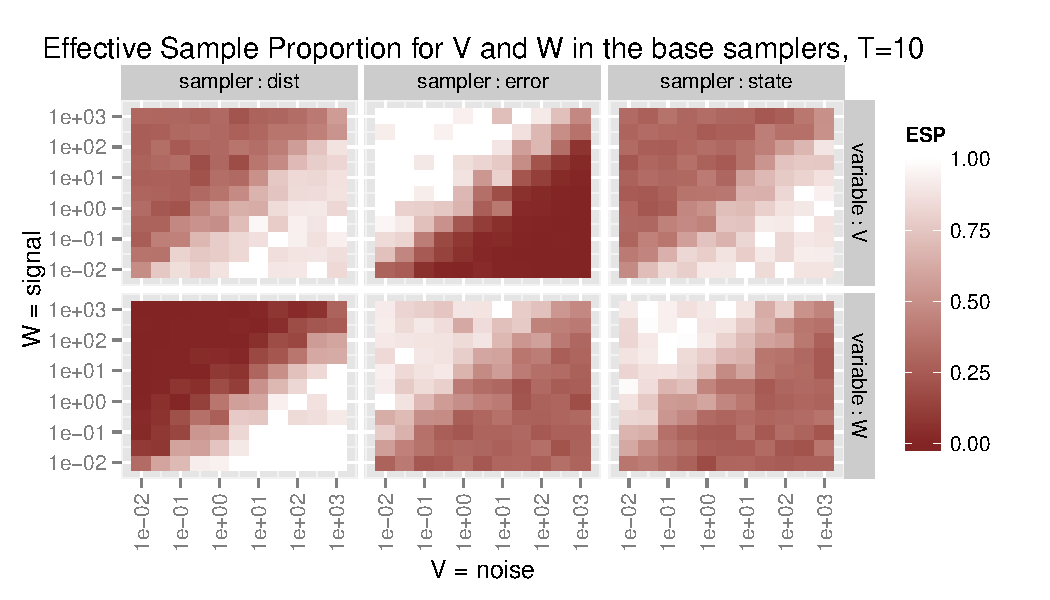
\includegraphics[width=1\textwidth]{figure/baseESplotT10} 

\end{knitrout}

\end{frame}

\begin{frame}
    \frametitle{Simulation Results for the Base Algorithms, $T=1000$}
\begin{knitrout}\footnotesize
\definecolor{shadecolor}{rgb}{0.969, 0.969, 0.969}\color{fgcolor}
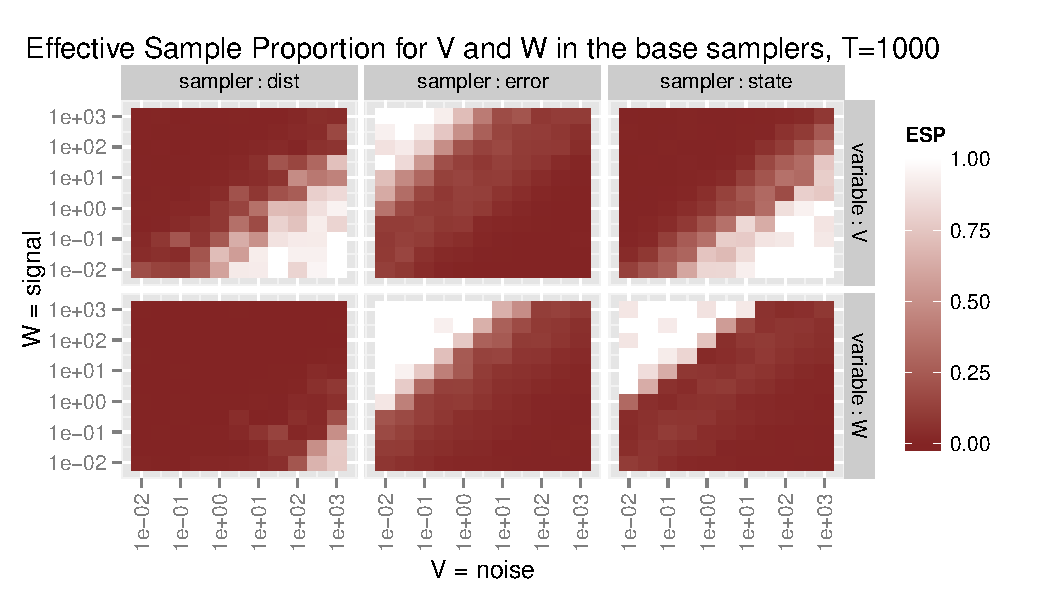
\includegraphics[width=1\textwidth]{figure/baseESplotT1000} 

\end{knitrout}


\end{frame}

\begin{frame}
  \frametitle{Takeaways from Base Algorithm Simulations}
  When the signal-to-noise ratio ($W/V$) is low ($<1$), the scaled disturbance sampler has high $ESP$ for both $V$ and $W$; when it's high ($>1$), the scaled disturbance sampler has low $ESP$ for both $V$ and $W$.\\~\\
  
  When the signal-to-noise ratio ($W/V$) is low ($<1$), the scaled error sampler has high $ESP$ for both $V$ and $W$; when it's high ($>1$), the scaled error sampler has low $ESP$ for both $V$ and $W$.\\~\\
  
  The state sampler agrees with the scaled disturbance sampler about $V$ and with the scaled error sampler about $W$. It's at it's best for $(V,W)$ when the signal-to-noise ratio is near $1$.\\~\\
  
  Despite not being an SA-AA pair, $\gamma_{0:T}$ and $\psi_{0:T}$ make a nice beauty and the beast pair.
  
\end{frame}


\begin{frame}
  \frametitle{GIS and Alternating Algorithms for the Local Level Model}
There are four possible GIS algorithms and four corresponding alternating algorithms:
\begin{table}[h]
  \centering
  \scalebox{.9}{
  \begin{tabular}{|l|cccc|}\hline
    Alternating: & State + Dist & State + Error & Dist + Error & Triple\\
    GIS: & State + Dist & State + Error & Dist + Error & Triple\\
    \hline
  \end{tabular}
  }
  \label{table:sams}
\end{table}
\pause

The State-Dist interweaving sampler, for example:
\begin{enumerate}
  \item Draw $\theta_{0:T}$ from $p(\theta_{0:T}|V^{(k)},W^{(k)},y_{1:T})$ using FFBS.
  \item Draw $(V,W)$ from $p(V,W|\theta_{0:T}, y_{1:T})$.
  \item Update $\gamma_{0:T}$ using $\theta_{0:T}$ and $(V,W)$.
  \item Draw $V^{(k+1)}$ from $p(V|\gamma_{0:T}, W, y_{1:T})$.
  \item Draw $W^{(k+1)}$ from $p(W|\gamma_{0:T}, V^{(k+1)}, y_{1:T})$, i.e. the same difficult density from before.\\~\\
\end{enumerate}
\pause
  The State-Dist alternating sampler would replace step 3 with a draw from $p(\gamma_{0:T}|V,W,y_{1:T})$.
\end{frame}

\begin{frame}
    \frametitle{Simulation Results for the GIS Algorithms, $T=10$}
    
\begin{knitrout}\footnotesize
\definecolor{shadecolor}{rgb}{0.969, 0.969, 0.969}\color{fgcolor}
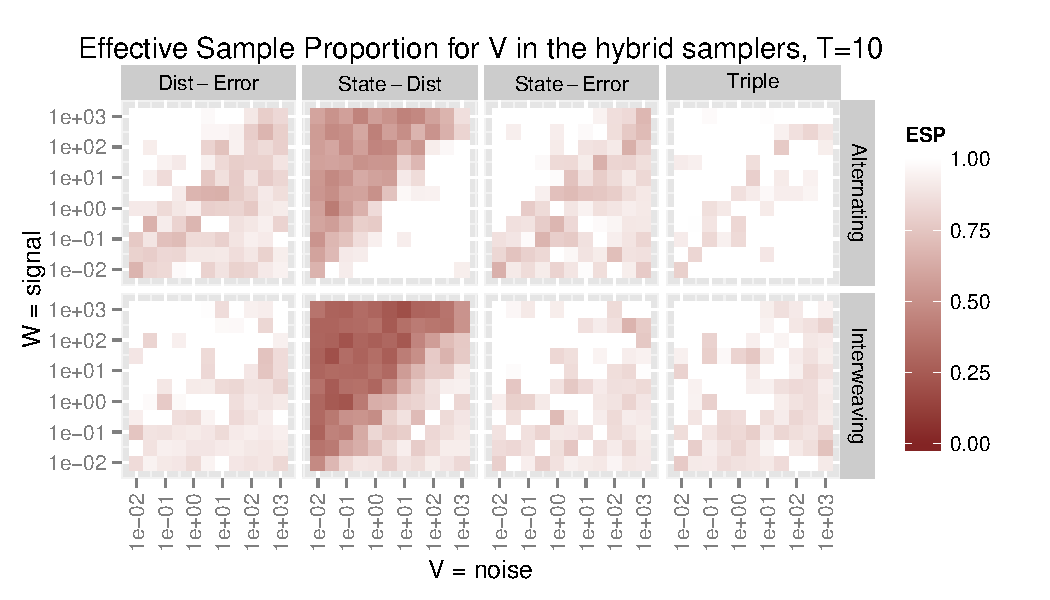
\includegraphics[width=1\textwidth]{figure/altintESplotT10-1} 

\end{knitrout}


\end{frame}

\begin{frame}
    \frametitle{Simulation Results for the GIS Algorithms, $T=10$}
    
\begin{knitrout}\footnotesize
\definecolor{shadecolor}{rgb}{0.969, 0.969, 0.969}\color{fgcolor}
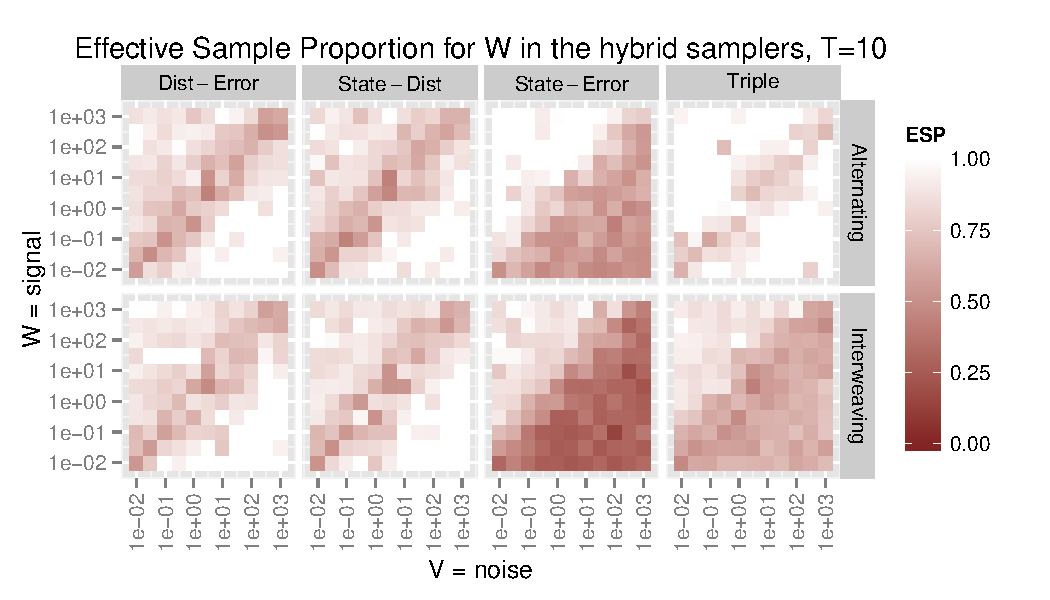
\includegraphics[width=1\textwidth]{figure/altintESplotT10-2} 

\end{knitrout}

\end{frame}

\begin{frame}
    \frametitle{Simulation Results for the GIS Algorithms, $T=1000$}
    
\begin{knitrout}\footnotesize
\definecolor{shadecolor}{rgb}{0.969, 0.969, 0.969}\color{fgcolor}
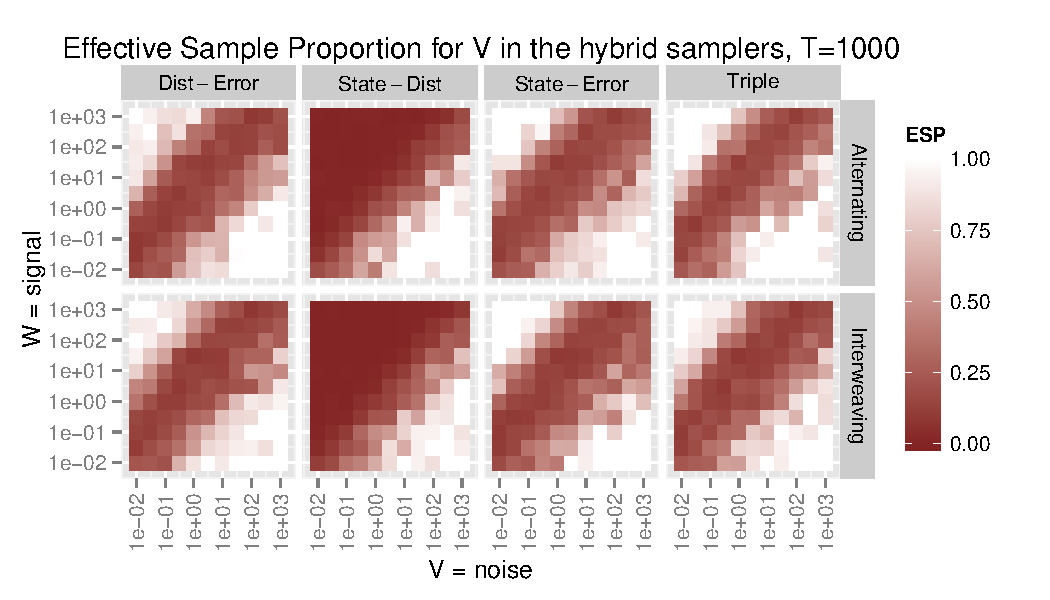
\includegraphics[width=1\textwidth]{figure/altintESplotT1000-1} 

\end{knitrout}


\end{frame}

\begin{frame}
    \frametitle{Simulation Results for the GIS Algorithms, $T=1000$}
    
\begin{knitrout}\footnotesize
\definecolor{shadecolor}{rgb}{0.969, 0.969, 0.969}\color{fgcolor}
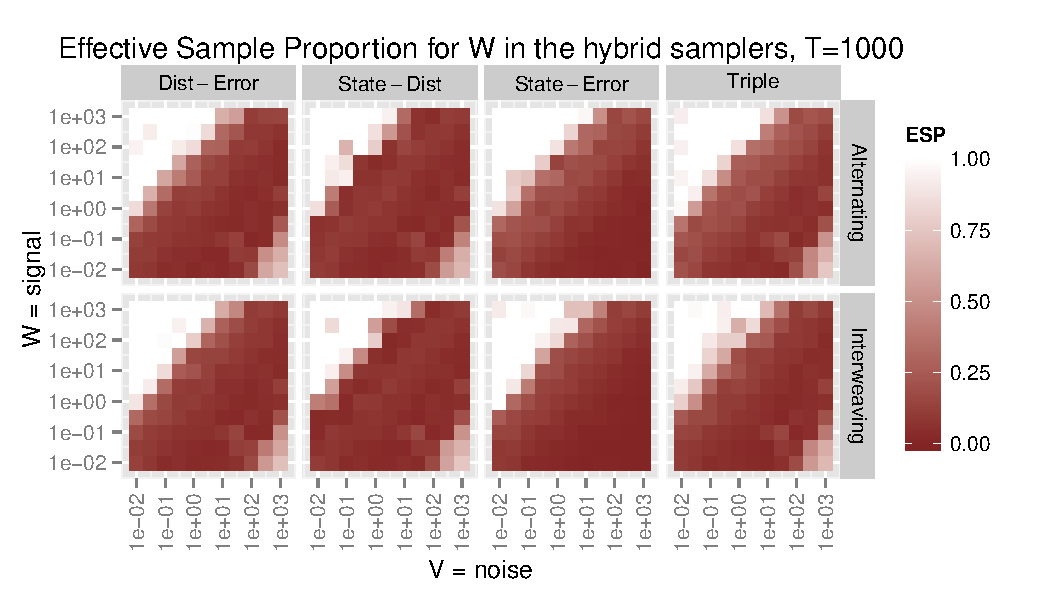
\includegraphics[width=1\textwidth]{figure/altintESplotT1000-2} 

\end{knitrout}

\end{frame}

\begin{frame}
  \frametitle{Takeaways from GIS Algorithm Simulations}
  For $T$ large enough, alternating or interweaving doesn't make a difference for ESP (but interweaving is less computationally expensive).\\~\\
  
  The Dist-Error interweaving algorithm and the Triple interweaving algorithm appear to have identical ESPs.\\~\\
\pause  
  The ``beauty and the beast'' intuition works for any given parameter, i.e. for $W$, the Dist-Error and State-Dist algorithms have the best ESP, but the State-Error algorithms has worse ESP in some regions of the parameter space.\\~\\
  
  For the reasonable areas of the parameter space ($W/V$ not too small or large), there are still major mixing problems.
\end{frame}

\begin{frame}
  \frametitle{Partial CIS for the Local Level Model}
  Recall $\theta_{0:T}$ is SA for $W|V$ and both $\gamma_{0:T}$ and $\psi_{0:T}$ are AA for $(V,W)$. So all we need is a SA for $V|W$ for a CIS algorithm.\\~\\
\pause  
  This appears hard to find at first glance, instead we can try partial CIS, i.e. an algorithm which only interweaves in one of the Gibbs steps:
  \begin{enumerate}
  \item Draw $\theta_{0:T}$ from $p(\theta_{0:T}|V^{(k)},W^{(k)},y_{1:T})$ using FFBS.
  \item Draw $V^{(k+1)}$ from $p(V|W^{(k)},\theta_{0:T},y_{1:T})$
  \item Draw $W$ from $p(W|V^{(k+.5)},\theta_{0:T},y_{1:T})$
  \item Update $\gamma_{0:T}$ where $\gamma_0=\theta_0$ and $\gamma_t=(\theta_t-\theta_{t-1})/\sqrt{W}$.
  \item Draw $W^{(k+1)}$ from $p(W|V^{(k+1)},\gamma_{0:T},y_{1:T})$\\~\\
  \end{enumerate}
  Note that we have to use $\gamma_{0:T}$ in step 4, otherwise steps 5 and 3 would be identical draws because $p(W|V,\theta_{0:T},y_{1:T})=p(W|V,\psi_{0:T},y_{1:T})$.
\end{frame}

\begin{frame}
  \frametitle{Full CIS for the Local Level Model}
  For $t=1,2,...,T$ define
  \begin{align*}
    \tilde{\gamma}_t & = \frac{\sqrt{W}}{\sqrt{V}}\gamma_t = \frac{\theta_t - \theta_{t-1}}{\sqrt{V}} = \frac{w_t}{\sqrt{V}}\\
  \end{align*}
  with $\tilde{\gamma}_0=\gamma_0=\theta_0$.\\~\\
  \pause
  
  The model written in terms of $\tilde{\gamma}_{0:T}$ is
  \begin{align*}
  y_t|\tilde{\gamma}_{0:T}, V, W &\stackrel{ind}{\sim} N(\tilde{\gamma}_0 + \sqrt{V}\textstyle\sum_{s=1}^{t-1}\tilde{\gamma}_s, V)\\
  \tilde{\gamma}_t|V,W &\stackrel{iid}{\sim} N(0, W/V)
\end{align*}
So $\gamma_{0:T}$ \& $\tilde{\gamma}_{0:T}$ make a AA-SA pair for $W|V$
\end{frame}


\begin{frame}
  \frametitle{Full CIS for the Local Level Model}
  For $t=1,2,...,T$ define
  \begin{align*}
    \tilde{\psi}_t & = \frac{\sqrt{V}}{\sqrt{W}}\psi_t = \frac{y_t - \theta_{t}}{\sqrt{W}} = \frac{v_t}{\sqrt{W}}\\
  \end{align*}
  with $\tilde{\psi}_0=\psi_0=\theta_0$.\\~\\
  \pause
  
  The model written in terms of $\tilde{\psi}_{0:T}$ is
  \begin{align*}
  y_t|\tilde{\psi}_{0:T}, y_{0:t-1}, V, W & \sim N(y_{t-1} + \sqrt{W}(\tilde{\psi}_t - \tilde{\psi}_{t-1}), W)\\
  \tilde{\psi}_t|V,W &\stackrel{iid}{\sim}N(0,V/W)
\end{align*}
except for $t=1$, the mean of the system equation is $\sqrt{W}\tilde{\psi}_1 - \tilde{\psi}_0$.\\~\\

So $\psi_{0:T}$ \& $\tilde{\psi}_{0:T}$ make a AA-SA pair for $V|W$
\end{frame}

\begin{frame}
    \frametitle{Full CIS for the Local Level Model}
It turns out that
\begin{align*}
  p(W|\tilde{\gamma}_{0:T}, V, y_{1:T}) &= p(W|\theta_{0:T}, V, y_{1:T})\\
  p(V|\tilde{\psi}_{0:T}, W, y_{1:T}) &= p(V|\theta_{0:T}, W, y_{1:T})
\end{align*}
\pause 
which makes full CIS look like an extention of partial CIS:
\begin{enumerate}
  \item Draw $\theta_{0:T}$ from $p(\theta_{0:T}|V^{(k)},W^{(k)},y_{1:T})$.
  \item Draw $V$ from $p(V|W^{(k)}, \theta_{0:T}, y_{1:T})$.
  \item Update $\psi_{0:T}$ from $V$ and $\theta_{0:T}$.
  \item Draw $V^{(k+1)}$ from $p(V|W^{(k)}, \psi_{0:T}, y_{1:T})$.
  \item Update $\theta_{0:T}$ from $V^{(k+1)}$ and $\psi_{0:T}$.
  \item Draw $W$ from $p(W|V^{(k+1)}, \theta_{0:T}, y_{1:T})$.
  \item Update $\gamma_{0:T}$ from $W$ and $\theta_{0:T}$.
  \item Draw $W^{(k+1)}$ from $p(W|V^{(k+1)}, \gamma_{0:T}, y_{1:T})$.
\end{enumerate}
\end{frame}





\begin{frame}
\frametitle{Simulation Results for CIS Algorithms, $T=10$}
\begin{knitrout}\footnotesize
\definecolor{shadecolor}{rgb}{0.969, 0.969, 0.969}\color{fgcolor}
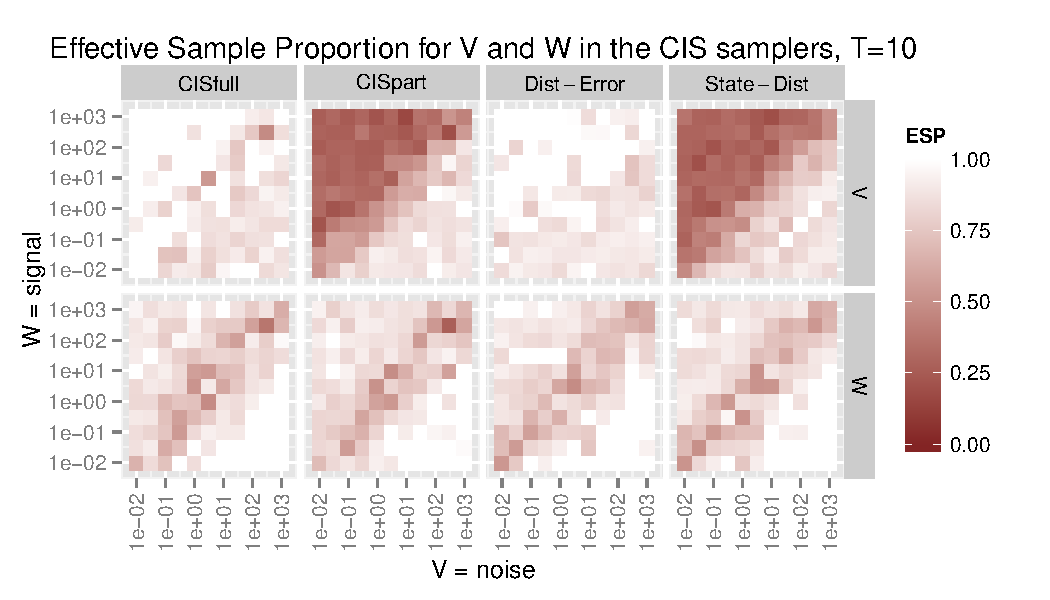
\includegraphics[width=1\textwidth]{figure/cisESplotT10} 

\end{knitrout}

\end{frame}

\begin{frame}
\frametitle{Simulation Results for CIS Algorithms, $T=1000$}

\begin{knitrout}\footnotesize
\definecolor{shadecolor}{rgb}{0.969, 0.969, 0.969}\color{fgcolor}
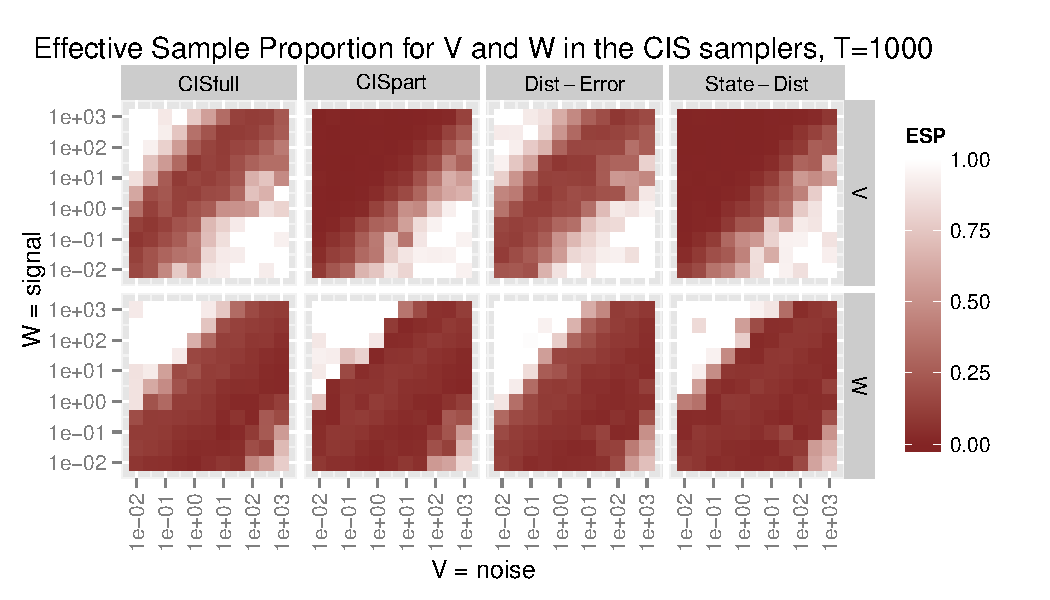
\includegraphics[width=1\textwidth]{figure/cisESplotT1000} 

\end{knitrout}


\end{frame}
 
\begin{frame}
   \frametitle{Main Takeaways from CIS Simulations}
   Full CIS looks identical to Dist-Error GIS and Partial CIS looks identical to State-Dist GIS.\\~\\
   
   This suggests that another Partial CIS algorithm exists that implicitly uses $\tilde{\psi}_{0:T}$ instead of $\tilde{\gamma}_{0:T}$ and behaves identically to the State-Error GIS algorithm.\\~\\
   \pause
   
   Upshot: there's no good reason to use CIS instead of GIS in the local level model since CIS requires more computation.\\~\\
\end{frame}

\begin{frame}
\frametitle{Recommendations in the Local Level Model}
If $T$ is small ($<100$), use the state sampler.\\~\\

If $T$ is large, use the Dist-Error GIS sampler, but spend some time obtaining efficient draws from the complex densities --- $p(W|\gamma_{0:T},V,y_{1:T}$ and $p(V|\psi_{0:T},W,y_{1:T})$.\\~\\
\pause

Possibly use metropolis steps for $(V,W)$ jointly in the Dist-Error GIS sampler --- untested, but likely has decent mixing properties and avoids the expensive sampling steps.
\end{frame}

\begin{frame}
  \frametitle{Generalizations to other DLMS}
Suppose $y_t$ and $\theta_t$ are now vectors and
\begin{align*}
  y_t|\theta_{0:T} & \stackrel{ind}{\sim} N(F_t\theta_t, V)\\
  \theta_t|\theta_{0:t-1} & \sim N(G_t\theta_{t-1}, W)
\end{align*}
with $F_t$, $G_t$ known matricies for $t=1,2,...,T$ and $V$, $W$ unknown covariance matricies.\pause Then for $t=1,2,...,T$:
\begin{align*}
  \gamma_t & = W^{-\frac{1}{2}}(\theta_t - G_t\theta_{t-1})\\
  \psi_t & = V^{-\frac{1}{2}}(y_t - F_t\theta_t)
\end{align*}
Note $dim(\gamma_t)=dim(\theta_t)$ and $dim(\psi_t)=dim(y_t)$ while in general $dim(\theta_t)\neq dim(y_t)$.\\~\\
\pause
Multivariate analogue of $W/V$: $|W|/|V|$? Ratio of eigenvalues?
\end{frame}
\begin{frame}[allowframebreaks]
        \frametitle{References}
        \bibliographystyle{plainnat}
        \bibliography{../mcmcex.bib}
\end{frame} 


\end{document}

